\documentclass[../../document.tex]{subfiles}

\begin{document}
    \section{Linear Context-Free Rewriting Systems}\label{sec:grammar:lcfrs}
    In linear context-free rewriting systems \defabrv{\lcfrs}{\abrv{lcfrs}}, each rule composes a tuple of strings from arguments that are string tuples as well.
    The first definition formalizes the notation for such compositions using variables that specify an argument in a subscript and one of its components in the superscript.
    The sets of compositions are restricted such that the variables occur ordered according to their sub- and superscripts, and no variables for consecutive components of the same argument occur next to each other.
    These restrictions enforce a normal form for \abrv{lcfrs} that matches the properties of grammars extracted from treebanks.
    The normal form itself, however, is not restrictive: For every \abrv{lcfrs}, there is an equivalent \abrv{lcfrs} in normal form (\citealp[Lemma~2.2]{SekMatFujKas91}; and \citealp[Definition~7.2]{Kal10}).

    \begin{definition}[Compositions]\label{def:lcfrs:comp}
        We fix a set of variables \(\X = \big\{ \x_i^j \mid i, j \in \DN_+ \big\}\) and the \({\DN_+}^*\)-indexed family of finite subsets \(\X_{s_1\cdots s_k} = \big\{ \x_i^j \mid i \in [k], j \in [s_i] \big\}\) for each \(k \in \DN\), and \(s_1, \ldots, s_k \in \DN_+\).
        Let \(\varSigma\) be a set that is disjoint from \(\X\) and \(s \in \DN_+\).
        An \deflab<composition>{\abrv{lcfrs} composition} over \(\varSigma\) of length \(s\) is a sequence \((u_1, \ldots, u_s)\) where the elements \(u_1, \dots, u_s \in (\varSigma \cup \X)^+\) are non-empty sequences over variables in \(X\) and symbols in \(\varSigma\) such that
        \begin{compactenum}
            \item each variable in \(\X\) occurs at most once in \(u_1 \cdots u_s\),
            \item for each \(i \in \DN_+\), if the variable \(\x_{i+1}^1\) occurs in the composition, then \(\x_i^1\) occurs to the left of it in \(u_1 \ldots u_s\),
            \item for each pair \(i, j \in \DN_+\), if the variable \(\x_i^{j+1}\) occurs in the composition, then \(\x_i^j\) occurs to the left of it in \(u_1 \ldots u_s\),
            \item there is no pair \(i, j \in \DN_+\) such that \(\x^j_i\x^{j+1}_i\) is a subsequence in any of \(u_1, \ldots, u_s\).
        \end{compactenum}
        For each \(k\in \DN\) and \(s, s_1, \ldots, s_k \in \DN_+\), the identifier \(\C^\varSigma_{(s_1\cdots s_k, s)}\) denotes the set of all \abrv{lcfrs} compositions over \(\varSigma\) of length \(s\) that contain the variables in \(\X_{s_1 \cdots s_k}\) exactly once and no other variable in \(\X \setminus \X_{s_1\cdots s_k}\).
        \(\C^\varSigma\) denotes the set of all \abrv{lcfrs} compositions over \(\varSigma\) of any length.

        Consider such a composition \((u_1, \ldots, u_s) \in \C^\varSigma_{(s_1\cdots s_k s)}\) for some naturals \(k \in \DN\), \(s\in \DN_+\) as well as \(s_1, \ldots, s_k \in \DN_+\).
        We associate a function, denoted by \(\sem{(u_1, \ldots, u_s)}\), from \(k\) string tuples, where the \(i\)th tuple is of length \(s_i\), to a string tuple of length \(s\) with the composition \((u_1, \ldots, u_s)\).
        For a sequence of arguments \(\big(v_i = (v_i^j \in \varSigma^* \mid j \in [s_i]) \mid i \in [k]\big)\), the result is the string tuple \(
        \sem{(u_1, \ldots, u_s)}(v_1, \ldots, v_k) = (u_1[\phi], \ldots, u_s[\phi])
        \) where \(\phi\) is the \(\X_{s_1 \cdots s_k}\)-indexed family \((\phi_{x_i^j} = v_i^j \mid i \in[k], j \in [s_i])\).
        In simple terms, this function replaces each occurring variable of the form \(\x_i^j\) in \(u_1, \ldots, u_s\) with the \(j\)th component of the \(i\)th argument.
    \end{definition}

    \begin{example}\label{ex:lcfrs:comp}
        Consider an alphabet \(\Sigma=\{\tn{A}, \tn{hearing}, \tn{is}, \tn{scheduled}, \tn{on}, \tn{the}, \tn{issue}, \tn{today}\}\) and the following compositions:
        \begin{align*}
            c_1 &= (\tn{A}), & c_2 &= (\tn{today}), & c_3 &= (\tn{issue}) && \in \C^\Sigma_{(\varepsilon, 1)} \\
            c_4 &= (\tn{the} \, \x_1^1), & c_5 &= (\x_1^1 \, \tn{hearing}) & & && \in \C^\Sigma_{(1,1)} \\
            c_6 &= (\x_1^1 \, \tn{is} \, \x_1^2) && && && \in \C^\Sigma_{(2,1)} \\
            c_7 &= (\x_1^1, \tn{on} \, \x_2^1) && && && \in \C^\Sigma_{(1\,1,2)}   \\
            c_8 &= (\x_1^1, \tn{scheduled} \, \x_1^2 \, \x_2^1) && && && \in \C^\Sigma_{(2\,1,2)}
        \end{align*}

        The subscript in the family of compositions \(\C^\Sigma\) determines the arities as well as the shape of arguments for the associated functions.
        For instance, the function \(\sem{c_1}\) associated with \(c_1 \in \C^\Sigma_{(\varepsilon, 1)}\) takes no arguments (it is constant) and yields a single string,
        the function for \(c_8 \in \C^\Sigma_{(2\,1, 2)}\) takes two arguments: a sequence of strings of length 2 and a singleton sequence of strings, and gives a sequence of length 2 as a result.
        The following equation shows an application of the function \(\sem{c_8}\) to two sequences of strings: 
        \begin{multline*}
            \sem{c_8}\Big( \; \big( \tn{A hearing}, \: \tn{on the issue} \big), \, \big( \tn{today} \big) \; \Big)
            \\= \big( \tn{A hearing}, \: \tn{scheduled on the issue today} \big) \text{.}
        \end{multline*}

        The following sequence of terms denotes a series of such applications:
        \begin{align*}
            \sem{c_7}\Big( \; \sem{c_5}\big(\,\sem{c_1}()\,\big), \: \sem{c_4}\big(\,\sem{c_3}()\,\big) \; \Big)
            =& \sem{c_7}\Big( \; \sem{c_5}\big(\tn{A}\big), \: \sem{c_4}\big(\tn{issue}\big) \; \Big) \\
            =& \sem{c_7}\Big( \; (\tn{A hearing}), \: (\tn{the issue}) \; \Big) \\
            =& (\tn{A hearing}, \: \tn{on the issue}) \text{.}
        \end{align*}
    \end{example}

    \begin{definition}[\abrv{Lcfrs} Rules and Grammars]
        Let \(\varSigma\) and \(N\) be sets and \(\mathit{fo}\colon N \to \DN_+\) a function.
        An \deflab<rule>{\abrv{lcfrs} rule} (with terminals in \(\varSigma\), nonterminals in \(N\), and fanout \(\mathit{fo}\)) is of the form \(A \to c\,(B_1, \ldots, B_k)\) where \(k \in \DN\), \(A, B_1, \ldots, B_k \in N\) and \(c \in \C^\varSigma_{(\mathit{fo}(B_1) \cdots \mathit{fo}(B_k), \mathit{fo}(A))}\) is a composition.
        \(A\) is called the left-hand side (\abrv{lhs}) nonterminal and \(B_1, \ldots B_k\) are the right-hand side (\abrv{rhs}) nonterminals, \(c\) is the composition of the rule.
        The natural \(k\) is the \deflab<rank>{rank of an \abrv{lcfrs} rule}[rank] of the rule.
        In the case of \(k = 0\), the rule is slightly abbreviated by dropping the trailing parentheses.
        The identifier \(\Rules^{\varSigma, N, \mathit{fo}}\) denotes the set of all such \abrv{lcfrs} rules.

        A \deflab{\lcfrs} \defabrv{\lcfrs}{\abrv{lcfrs}} is a tuple \(G=(N, \varSigma, S, R)\) where
        \begin{compactenum}
            \item \(N\) is a set (\emph{nonterminals}),
            \item \(\varSigma\) is a set (\emph{terminals}),
            \item \(S \subseteq N\) (initial non-terminals),
            \item \(R\) is a finite subset of \(\R^{\varSigma, N, \fanout_G}\) where \(\fanout_G\) is an implicit function that maps each nonterminal to a positive integer matching the above requirement. For each \(A \in N\), the value \(\fanout_G(A)\) is called \deflab<fanout>{fanout of a nonterminal}[fanout of \(A\)].
        \end{compactenum}
    \end{definition}

    The fanout function \(\fanout_G\) ensures that the variables occurring in the compositions are consistent with the tuples that can be computed with rules for the \abrv{rhs} nonterminals.
    The lengths of the compositions occurring in the rules with the same \abrv{lhs} nonterminal are thus equal.

    \begin{definition}[\abrv{Lcfrs} Grammar Forms]
        We distinguish rules and grammar instances of the following form:
        \begin{compactitem}
            \item A rule of rank zero, one and two is called \deflab{nullary grammar rule}[nullary], \deflab<unary>{unary grammar rule}[unary] and \deflab<binary>{binary grammar rule}[binary], respectively.
            \item An \abrv{lcfrs} containing only nullary, unary, and binary rules is called \deflab<binary>{binary grammar}[binary].
            \item A rule whose composition contains exactly one terminal in \(\varSigma\) is called \deflab<lexical>{lexical grammar rule}[lexical].
            \item An \abrv{lcfrs} containing only lexical rules is called \deflab<lexical>{lexical grammar}[lexical].
            \item A rule whose composition contains no terminal at all is called \deflab{non-lexical grammar rule}[non-lexical].
%            \item
%                An \abrv{lcfrs} that contains only lexical nullary rules and non-lexical rules of rank \(\ge 1\) and whose initial nonterminals do not occur in any rule's \abrv{rhs} is called \deflab<\lcfrs>[lcfrs:simple]{simple}.
        \end{compactitem}
    \end{definition}

    \begin{example}[Continues \cref{ex:lcfrs:comp}]\label{ex:lcfrs:rules}
        Consider the alphabet of nonterminal symbols \(\mathrm{N} = \{\nt{v}, \nt{v}_2, \nt{n}, \nt{n}_2, \nt{p}, \nt{d}\}\) and the \abrv{lcfrs} \(\mathrm{G} = (\mathrm{N}, \Sigma, \{\nt{v}\}, \mathrm{R})\) with
        \begin{align*}
            \mathrm{R} = \big\{\;
            \nt{d} &\to (\tn{A}), &\nt{n} &\to (\tn{issue}), &\nt{n} &\to (\tn{today}), &\\
            \nt{n} &\to (\x_1^1 \, \tn{hearing})\:(\nt{d}), &\nt{p} &\to (\tn{the}\,\x_1^1)\:(\nt{n}), \\
            \nt{n}_2 &\to (\x_1^1, \tn{on} \, \x_2^1)\:(\nt{n}, \nt{p}), \\
            \nt{v}_2 &\to (\x_1^1, \tn{scheduled} \, \x_1^2 \, \x_2^1)\:(\nt{n}_2, \nt{n}), \\
            \nt{v} &\to (\x_1^1 \, \tn{is} \, \x_1^2)\:(\nt{v}_2)
            &&&&&\;\big\}
        \end{align*}
        The fanout for each nonterminal \(A\) determines the length of the composition with \abrv{lhs} \(A\) and the number of variables if \(A\) occurs in the \abrv{rhs} nonterminals of a rule.
        In the above example, the nonterminal symbols with subscript \(_2\), i.e., \(\nt{n}_2\) and \(\nt{v}_2\), are of fanout 2, and all others of fanout 1.
        The composition of the rule \(\nt{v}_2 \to (\x_1^1, \tn{scheduled} \, \x_1^2 \, \x_2^1)\:(\nt{n}_2, \nt{n})\) is of length \(\fanout_{\mathrm{G}}(\nt{v}_2) = 2\) and there are \(\fanout_{\mathrm{G}}(\nt{n}_2) = 2\) variables for the first \abrv{rhs} nonterminal and \(\fanout_{\mathrm{G}}(\nt{n}) = 1\) for the second.
    \end{example}

    \begin{definition}[Derivation]
        Let us consider an \abrv{lcfrs} \(G = (N, \varSigma, S, R)\).
        An \deflab<derivation>{\abrv{lcfrs} derivation} is a tree over rules in \(\T_R\) that satisfies the following conditions:
        \begin{compactitem}
            \item Each leaf is equipped with a nullary rule as a symbol.
            \item Each inner node is a rule with the same amount of \abrv{rhs} nonterminals as children in the tree such that the \(i\)th \abrv{rhs} nonterminal is the \(i\)th child's \abrv{lhs} nonterminal.
        \end{compactitem}
        The set of all \abrv{lcfrs} derivations is denoted by \(\derivs^R\).
        We also consider the \(N\)-indexed partition \((\derivs^R_A \mid A \in N)\) such that \(\derivs^R_A\) contains exactly the set of derivations in \(\derivs^R\) whose root is equipped with the \abrv{lhs} nonterminal \(A\).
    \end{definition}

    \begin{definition}[Yield]
        Consider a derivation \(d\) in \(\derivs^R\) of the form \(d = r\,(d_1, \ldots, d_k)\) where the root \(r\) is of the form \(A \to c\,(B_1, \ldots, B_k)\).
        The \deflab<yield>{yield of an \abrv{lcfrs} derivation}[yield of \(d\)] is defined recursively: \(\yield(d) = \sem{c}(\yield(d_1), \ldots, \yield(d_k))\).
        For each set of derivations \(D \subseteq \derivs^R\), we denote the set of all derivations for a given string \(w \in \varSigma^*\) by \(D(w) = \{d\in D \mid \yield(d) = w\}\).
    \end{definition}

    \begin{example}[Continues \cref{ex:lcfrs:comp,ex:lcfrs:rules}]\label{ex:lcfrs:deriv}\NoEndMark
        Let us consider the tree illustrated below:
            It is a derivation in the \abrv{lcfrs} \(\mathrm{G} = (N, \Sigma, \{\nt{v}\}, R)\) shown in the previous examples.
        Its root has the \abrv{lhs} nonterminal \(\nt{n}_2\), hence, the tree is an element of \(\derivs^R_{\nt{n}_2}\).
        The yield of \(d\) is the term over compositions computed in \cref{ex:lcfrs:comp}: \(\yield(d) = (\tn{A hearing}, \: \tn{on the issue})\).
        
        \null\hfill
        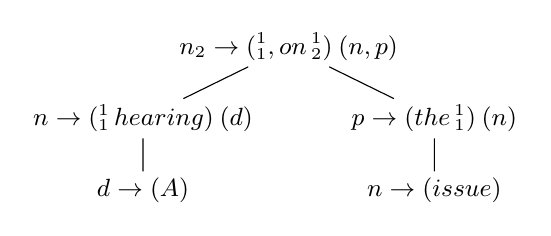
\begin{tikzpicture}[level distance=6ex, font=\small, sibling distance=3.7cm, inner sep=2pt]
            \node (root) {\(\nt{n}_2 \to (\x_1^1, \tn{on} \, \x_2^1)\:(\nt{n}, \nt{p})\)}
            child {node {\(\nt{n} \to (\x_1^1 \, \tn{hearing})\:(\nt{d})\)}
                child {node {\(\nt{d} \to (\tn{A})\)}}}
            child {node {\(\nt{p} \to (\tn{the}\,\x_1^1)\:(\nt{n})\)}
                child {node {\(\nt{n} \to (\tn{issue})\)}}};
        \end{tikzpicture}
        \hfill
        \exampleqed
    \end{example}

    During the extraction and parsing, \abrv{lcfrs} rules are instantiated with sentence positions \citep[Definition~6.8]{Kal10}.
    That is, instead of terminals that resemble objects in the sentence, we will assume matching sentence positions as lexical symbols in the rules.
    All derivations are assembled such that the compositions only concatenate consecutive sequences of positions.
    Each derivation is equivalent to a constituent tree that assumes the \abrv{lhs} nonterminals as inner nodes and the sentence positions as leaves.

    \begin{definition}[Position Instantiation]
        Let \(G = (N, \varSigma, S, R)\) be an \abrv{lcfrs}, and \(w = \sigma_1 \ldots \sigma_n\) a word of length \(n \in \DN_+\) over the same alphabet with \((\sigma_i \in \varSigma \mid i \in [n])\).
        Consider a rule \(r\in R\) of the form \(A \to c (B_1, \ldots, B_k)\); a rule \(r' \in \Rules^{[n],N,\fanout_G}\) that is equipped with positions in \(w\) as lexical symbols is called a \deflab{position instantiation} of \(r\) in \(w\) if it is obtained from \(r\) by replacing each lexical symbol \(\sigma\) in \(c\) with a position \(i \in [n]\) such that \(\sigma_i = \sigma\).
        The \abrv{lcfrs} \(G' = (N, [n], S, R')\) is called a \deflab{position instantiation}[position instantiation of \(G\) in \(w\)] if each rule in the set \(R'\) is a position instantiation of some rule \(r\in R\) in \(w\).

        A derivation \(d \in \derivs^{R'}\) is called \deflab<admissible>{admissible \abrv{lcfrs} derivation}[admissible], if its yield \(\yield(d)\) of the form \((s_1, \ldots, s_k)\) contains only contiguous sequences of positions in \(w\) and, for each \(i \in [k-1]\), the last position in \(s_i\) is at least by 2 smaller than the first position in \(s_{i+1}\).
        The \emph{set of admissible derivations in $R'$} is denoted as \(\aderivs^{R'}\).
    \end{definition}

    \begin{definition}[Constituent Structure for Derivation]
        Consider a position instantiation \((N, [n], S, R)\) of some \abrv{lcfrs} in a word \(w = \sigma_1 \ldots \sigma_n\) that is of length \(n\), and an admissible derivation \(d \in \aderivs^R\) of the form \(d = r\,(d_1, \ldots, d_k)\) where the root \(r\) is of the form \(A \to c\,(B_1, \ldots, B_k)\).
        We define the following \(k+1\) sequences of terminal symbols \(w_1, \ldots, w_{k+1} \in [n]^*\) that occur within the composition \(c\) as follows:
        \begin{compactitem}
                \item \(w_1\) is the sequence of terminal symbols occurring before the variable \(\x_1^1\) in \(c\),
                \item for each \(i \in \{2, \ldots, k\}\), \(w_i\) is the sequence of terminal symbols occurring between the variables \(\x_{i-1}^1\) and \(\x_i^1\) in \(c\), and
                \item \(w_{k+1}\) is the sequence of terminal symbols occurring after the variable \(\x_k^1\) in \(c\).
            \end{compactitem}
        Then the \deflab<constituent structure>{constituent structure for an \abrv{lcfrs} derivation}[constituent structure for \(d\)] is the tree \[
            \parse(d) = A(w_1, \parse(d_1), w_2, \parse(d_2), \ldots, w_k, \parse(d_k), w_{k+1}) \text{.}
        \]
    \end{definition}

    \begin{example}[Continues \cref{ex:lcfrs:comp,ex:lcfrs:rules}]\label{ex:lcfrs:instance}\NoEndMark
        Let us consider the \abrv{lcfrs} \(\mathrm{G}\) from the previous examples and an instantiation \(\mathrm{G'} = (N, [8], \nt{v}, R)\) of \(\mathrm{G}\) in the string following string (where the positions are illustrated as subscript to the right of each token): \[
            \tn{A}_1 \quad \tn{hearing}_2 \quad \tn{is}_3 \quad \tn{scheduled}_4 \quad \tn{on}_5 \quad \tn{the}_6 \quad \tn{issue}_7 \quad \tn{today}_8
        \]
        The left figure illustrates a derivation in the instantiated \abrv{lcfrs} \(\mathrm{G'}\).
        The right figure illustrates the constituent structure for \(d\).
    
        \null\hfill
        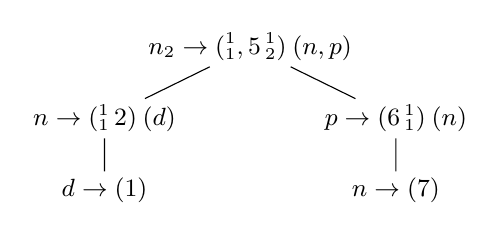
\begin{tikzpicture}[level distance=6ex, font=\small, sibling distance=3.7cm, inner sep=2pt]
            \node {\(\nt{n}_2 \to (\x_1^1, \tn{5} \, \x_2^1)\:(\nt{n}, \nt{p})\)}
            child {node {\(\nt{n} \to (\x_1^1 \, \tn{2})\:(\nt{d})\)}
                child {node {\(\nt{d} \to (\tn{1})\)}}}
            child {node {\(\nt{p} \to (\tn{6}\,\x_1^1)\:(\nt{n})\)}
                child {node {\(\nt{n} \to (\tn{7})\)}}};
        \end{tikzpicture}
        \hfill
        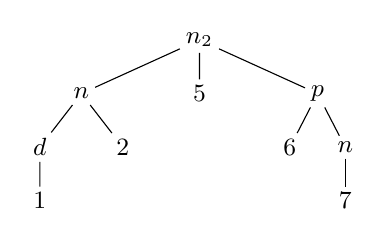
\begin{tikzpicture}[level distance=4.5ex, font=\small, inner sep=2pt]
            \node {\(\nt{n}_2\)}
            child {node {\(\nt{n}\)}
                [sibling distance=3em]
                child {node {\(\nt{d}\)}
                    child { node {\(\tn{1}\)}}}
                child {node {\(\tn{2}\)}}}
            child {node {\(\tn{5}\)}}
            child {node {\(\nt{p}\)}
                [sibling distance=2em]
                child {node {\(\tn{6}\)}}
                child {node {\(\nt{n}\)}
                    child { node {\(\tn{7}\)}}}};
        \end{tikzpicture}
        \hfill\exampleqed
    \end{example}

    The following definitions deal with extracting \abrv{lcfrs} rules from constituent structures.
    They are similar to the extraction of \emph{treebank grammars} by \citet{MaierSogaard08} but extend the procedure to accommodate lexical \abrv{lcfrs}.
    The extraction can be seen as a reversal of the previous definition of a constituent structure for a derivation.
    We start with an elementary definition that quantifies and assembles continuous sequences among sets of positions.

    \begin{definition}[Linearization]
        Let \(\pi \subset \DN_+\) be a finite and non-empty set.
        The \deflab{linearization} of \(\pi\) is the sequence of the greatest contiguous sequences within \(\pi\); that is, the sequence \((w_j \in \pi^+ \mid j \in [s])\) such that
        \begin{compactitem}
            \item \(s = |\{i \in \pi \mid i+1 \notin \pi\}|\) is the number of the greatest contiguous sets in \(\pi\),
            \item \(w_j\) is a contiguous sequence of increasing positive integers for each \(j \in [s]\),
            \item for each \(j \in [s]\), if \(i\) is the first (and therefore smallest) element in \(w_j\), then \(i-1 \notin \pi\); vice versa, if \(i\) is the last (and therefore greatest) element in \(w_j\), then \(i+1 \notin \pi\).
            % \item for each \(j \in [s-1]\), the last (and therefore greatest) element in \(w_j\) is at least two less than the first (and therefore least) element in \(w_{j+1}\).
        \end{compactitem}
        The positive integer \(s\) is called \deflab<fanout>{fanout of a set}[fanout of the set \(\pi\)].
    \end{definition}

    In the following definition, these sequences of continuous positions are used to define \abrv{lcfrs} compositions.
    It assumes a collection of sets of positions (in the yield of some bottom nodes) and one superseding set (in the yield of a top node).
    The composition is obtained from the linearization of the superseding set by substituting the sequences occurring in the collection with appropriate variables.

    \begin{definition}[Composition for Positions]
        Let \(k \in \DN\) be some natural, \((\pi_i \subset \DN_+ \mid i \in [k])\) a collection of mutually exclusive, finite and non-empty sets, and \(\pi_0 \supseteq \bigcup_{i \in [k]} \pi_i\) a finite and non-empty superset of their elements.
        The families \((s_i \mid i \in [0,k])\) and \((w_i^j \mid i \in [0,k], j \in [s_i])\) are the fanouts and linearizations of the sets \(\pi_0, \ldots, \pi_k\), respectively, such that \((w_i^j \mid j \in [s_i])\) identifies the linearization for \(\pi_i\).
        We define the \emph{\abrv{lcfrs} composition for \(\pi_0, \ldots, \pi_k\)}, denoted by \(\mathrm{comp}(\pi_0, \pi_1, \ldots, \pi_k)\), as the composition \((u_1, \ldots, u_{s_0}) \in \C^{\pi_0}_{(s_1\cdots s_k, s_0)}\) where each \(u_\ell\) is obtained from \(w_0^\ell\) by replacing each occurrence of a sequence \(w_i^j\) with the variable \(\x_i^j\).
    \end{definition}

    \begin{example}[Continues \Cref{ex:lcfrs:instance}]
        The top three inner nodes in the constituent structure shown in the previous example have the yields \(\pi_0 = \{1,2,5,6,7\}\) (at the root), \(\pi_1 = \{1,2\}\) (at position 1) and \(\pi_2 = \{6,7\}\) (at position 2).
        The linearization of \(\pi_0\) consists of the two sequences \(w_0^1 = 1\,2\) and \(w_0^2 = 5\,6\,7\), its fanout is \(s_0=2\).
        For the successor nodes the linearizations are \(w_1^1 = 1\,2\) and \(w_2^1 = 6\,7\), respectively, and their fanout is \(s_1 = s_2 = 1\).
        We obtain the composition for the three sets \(\pi_0\), \(\pi_1\) and \(\pi_2\) as follows:
            The first component \(u_1\) is obtained by replacing \(1\,2\) with the variable \(\x_1^1\) in \(w_0^1\) and the second component \(u_2\) analogously by replacing \(6\,7\) by \(\x_2^1\) in \(w_0^2\).
        It is \(\mathrm{comp}(\pi_0, \pi_1, \pi_2) = (u_1, u_2) = (\x_1^1, 5\,\x_2^1)\).
    \end{example}

    When \abrv{lcfrs} are used for parsing, they are often extended by weight structures.
    The following definition does not employ a general framework such as semirings, but assumes positive real values assigned to each rule and the sum operation to combine weight values within derivations.
    We interpret these values as scores or confidence values and understand higher values as better.
    This interpretation is equivalent to the usual probabilistic interpretation \citep[cf.][Viterbi semiring]{Goodman} with logarithmic values.

    \begin{definition}[Weighted \abrv{lcfrs}]
        Let \(G = (N, \varSigma, S, R)\) be an \abrv{lcfrs} and \(\weight \colon R \to \DR_{\ge 0}\) an assignment of a non-negative value to each rule in \(G\).
        We call \(\weight\) a \deflab{weight assignment} for \(G\) and the tuple \((G, \weight)\) a \deflab{weighted grammar}[weighted \abrv{lcfrs}].
        The weight of a derivation \(d \in \derivs^R\) is the sum over all positions' weights: \[ \weight(d) = \sum_{\rho \in \pos(d)} \weight(d(\rho))\text{.} \]
        The set of all best derivations in \(R\) for \(w \in \varSigma^*\) is \(\argmax_{d \in \derivs^R(w)} \weight(d)\).
        For each \(n\in \DN_+\), we extend this concept to the sequences of \(n\)-best derivations.
        The set of all \(n\)-best derivation sequences in \(R\) for \(w \in \varSigma^*\) is \(\argmax^{(n)}_{d \in \derivs^R(w)} \weight(d)\).
    \end{definition}
\end{document}